%!TEX root = ../Libro.tex
\section{Patrón de Arquitectura MVC}
Modelo-Vista-Controlador es un patrón de ingeniería del software que permite crear independencia entre la capa de interfaz, la capa de negocios y la capa de datos, facilitando el modificar la apariencia de la aplicación o las reglas del negocio sin afectar al resto. En el MVC el Modelo representa la información o la data de la aplicación y las reglas del negocio empleadas para manejarla, la Vista corresponde a los elementos de la interfaz del usuario como cuadros de texto, checkbox, etc. y el Controlador maneja los detalles correspondientes a la comunicación con el modelo de la aplicación.

\subsection {Elementos del patrón MVC}

\begin{itemize}
	\item \textbf{Modelo:} representa los datos y las reglas del negocio que manejan el acceso a esos datos. Generalmente el modelo se emplea como una aproximación al proceso original de diseño de la base de datos, por lo que las técnicas de modelado también aplican en la definición del modelo \citep{MVC_Java2002}.
	\item \textbf{Vista:} muestra el contenido del modelo. Accede a los datos del negocio, a través del modelo, y especifica que data debe ser mostrada. Es responsabilidad de la vista el mantener la consistencia en las presentaciones cuando el modelo cambia \citep{MVC_Java2002}.
	\item \textbf{Controlador:} lleva a cabo la traducción de la interacción con la vista a acciones que pueden ser ejecutadas por el modelo. Las acciones realizadas por el modelo incluyen el activar procesos del negocio o cambiar el estado del mismo. En base a la interacción del usuario y la salida de las operaciones del modelo, el controlador responde seleccionando una vista adecuada \citep{MVC_Java2002}.
\end{itemize}

El flujo de control para este patrón es \citep{MVC_WE2007}:
\begin{enumerate}
	\item El usuario interactúa con la interfaz.
	\item El controlador toma el evento de entrada de la interfaz con el usuario.
	\item El controlador notifica al modelo de la acción ejecutada por el usuario, que posiblemente resulta en un cambio en el estado del modelo.
	\item El controlador delega a los objetos de la vista la tarea de desplegar la interfaz de usuario. La vista obtiene sus datos del modelo para generar una interfaz que se adapte a los cambios del mismo. La vista toma los datos del modelo pero este no tiene conocimiento directo sobre la vista.
	\item Se esperan nuevas interacciones en la interfaz de usuario que inicien el ciclo nuevamente.
\end{enumerate}

\subsection {Ventajas}

\begin{itemize}
	\item \textbf{Permite la re-utilización de los componentes del modelo}\\
	La separación entre el modelo y la vista permite emplear varias vistas para un mismo modelo. Como consecuencia de esto los componentes del modelo son más fácil de implementar, probar y mantener, ya que todos los accesos se realizan a través de estos componentes.
	\item \textbf{Mayor facilidad para el soporte de nuevos tipos de clientes}\\
	Sólo es necesario crear nuevas vistas, incorporar alguna lógica en el controlador e integrarlo con la aplicación existente.
	\item \textbf{Facilidad en el diseño}\\
	Las aplicaciones web se han hecho más difíciles de diseñar que las aplicaciones tradicionales, el patrón MVC está siendo usado como una solución a esa dificultad.
\end{itemize}

\subsection {Desventajas}
\begin{itemize}
	\item \textbf{Incrementa la complejidad del diseño}\\
	El patrón introduce algunas clases extras para la separación del modelo, la vista y el controlador.
	\item \textbf{Cierta cohesión entre la vista y el controlador}\\
	Cualquier modificación en la vista suele significar un cambio en el controlador.
\end{itemize}

% 	
% \begin{figure}[ht]
% 	\centering
% 	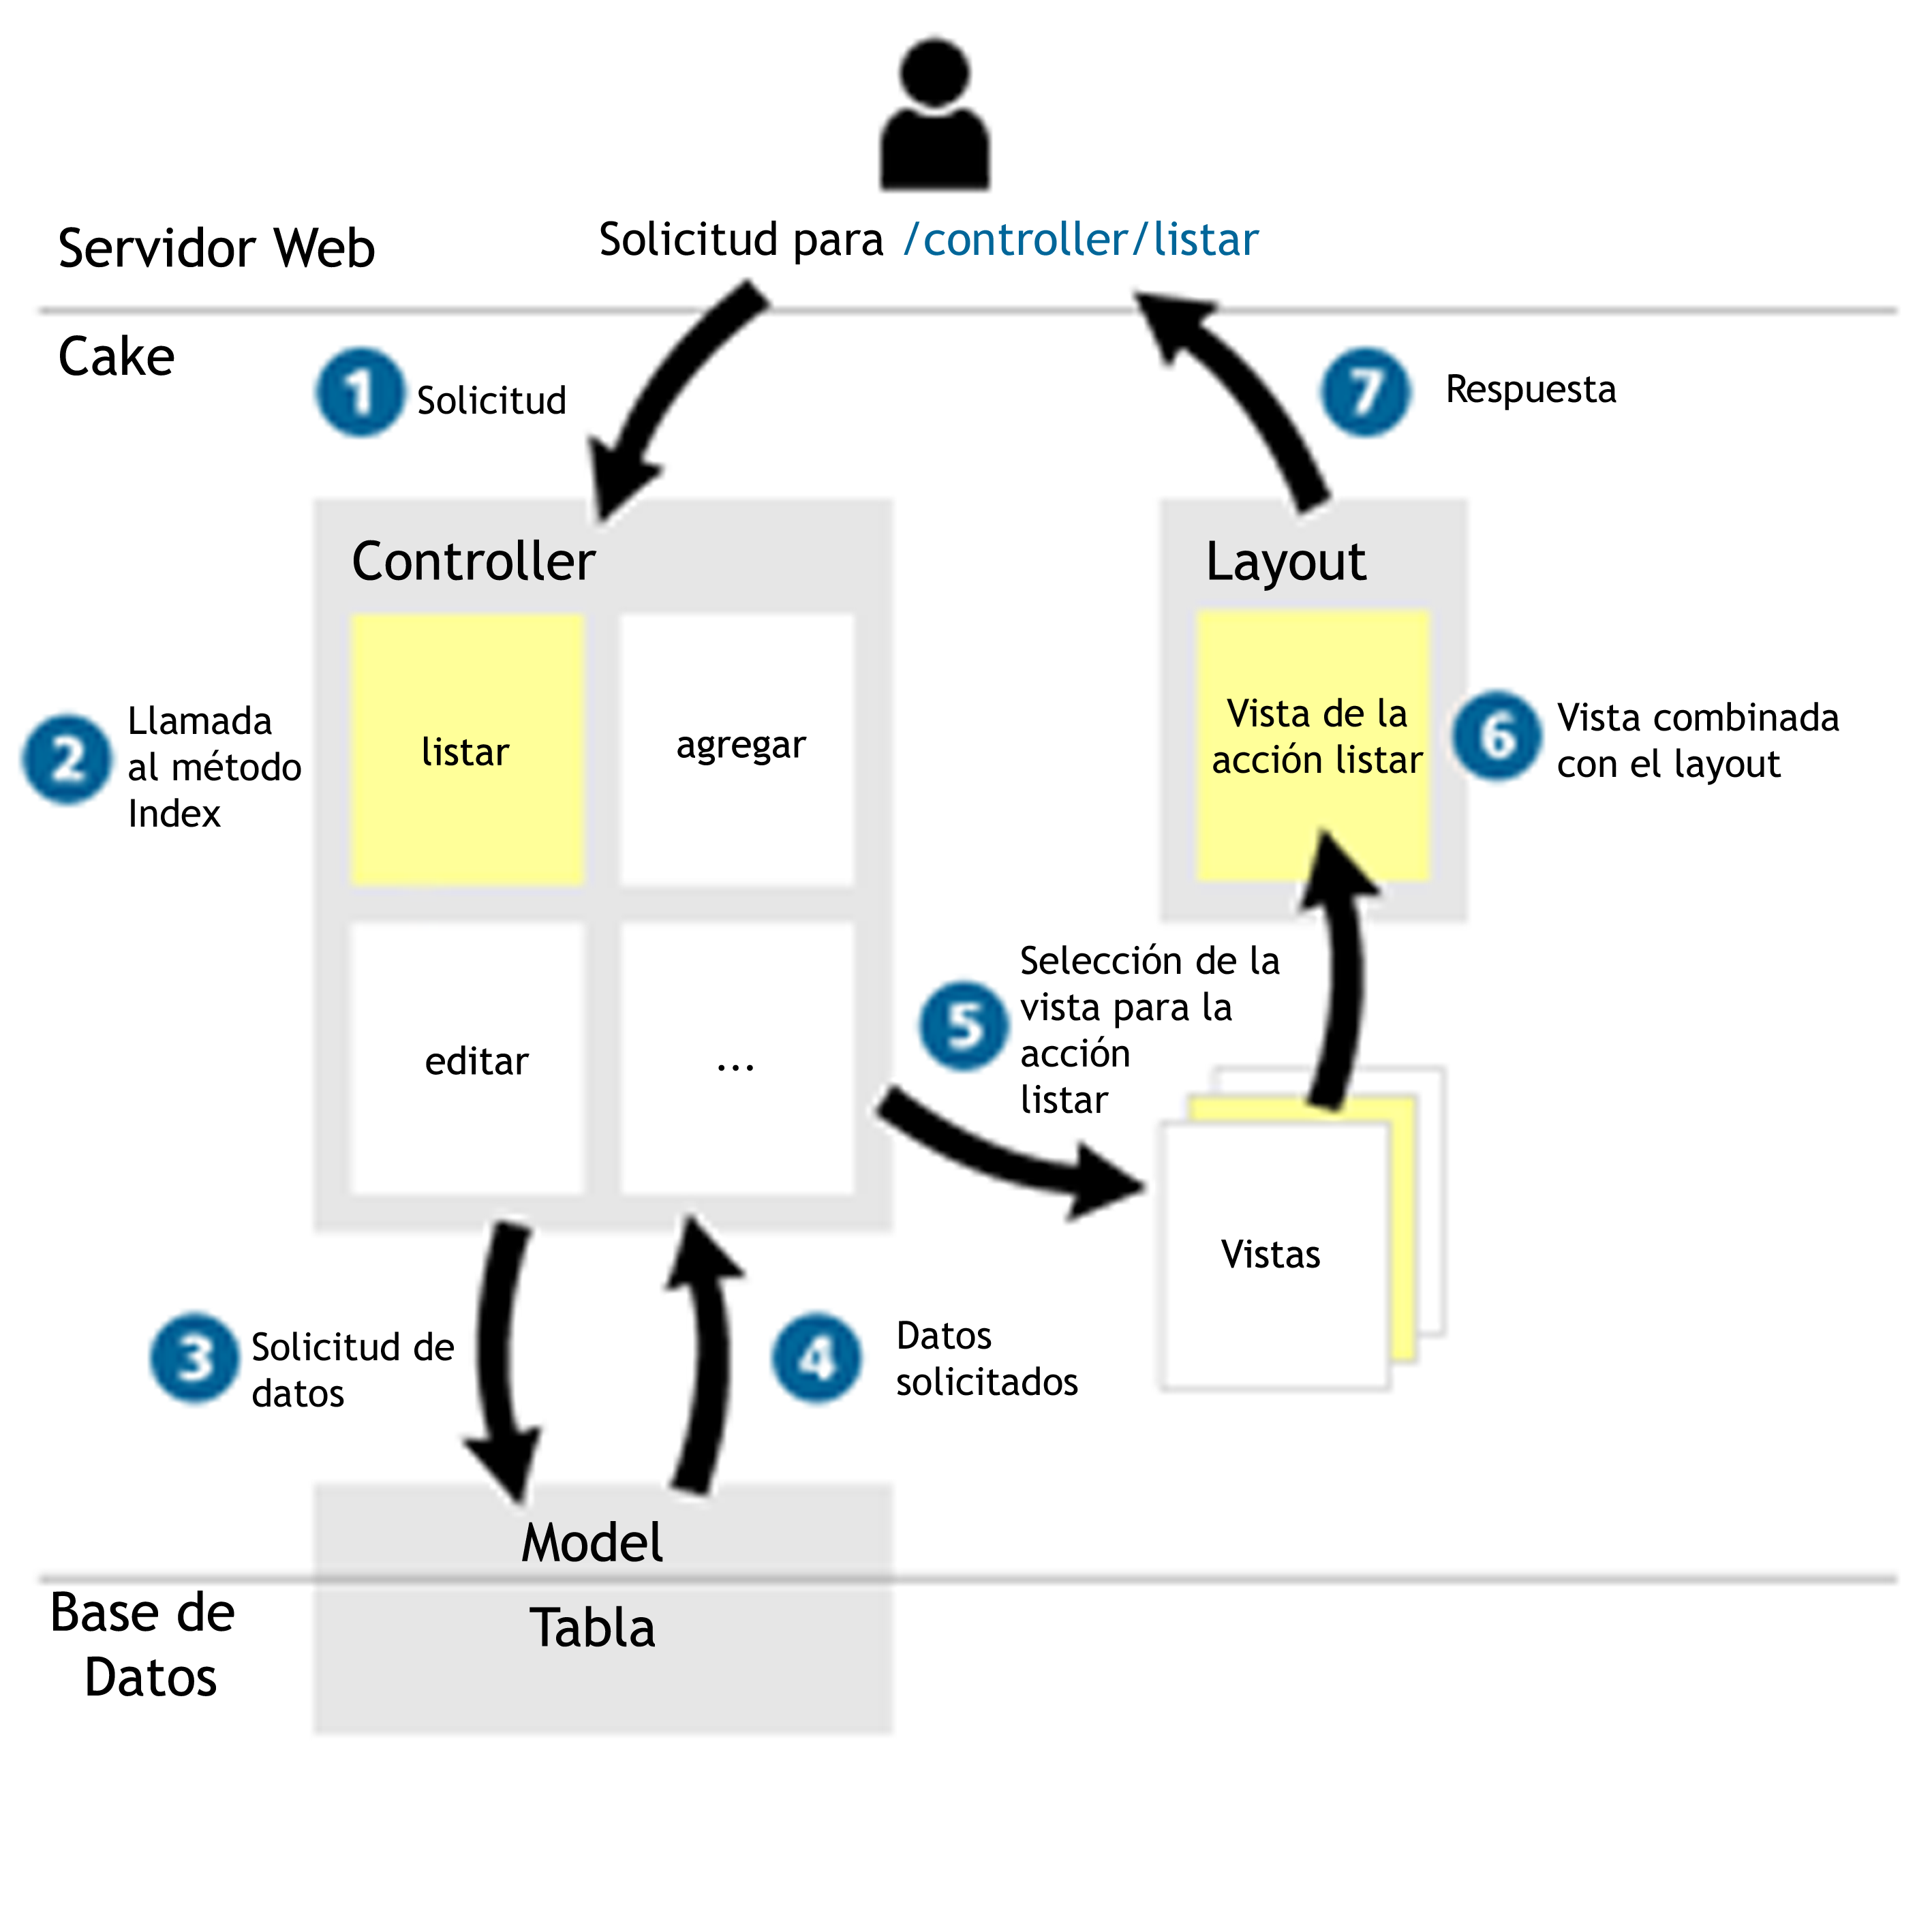
\includegraphics{imagenes/MVC_Cake.png}
% 	\caption{Diagrama del patrón MVC para Cake}
% 	\label{fig:mvc_cake}
% \end{figure}